% Use class option [extendedabs] to prepare the 1-page extended abstract.
\documentclass[extendedabs]{bmvc2k}
\usepackage[colorlinks = true,
            linkcolor = blue,
            urlcolor  = blue,
            citecolor = blue,
            anchorcolor = blue]{hyperref}
\usepackage{kotex}
% for the fancy \koTeX logo
\usepackage{kotex-logo}
\usepackage{mathtools}  % brings in amsmath, also some improvements
\usepackage{amssymb} % brings in amsfonts, incl \square
% Document starts here
\usepackage{graphicx}
\begin{document}


\title{lora with stable diffusion final report}
\addauthor{
Taehun Kim$^{1}$
}{}{1}

\addinstitution{
$^1$ Department of Computer Science and Engineering, Pusan National University.  
}
 

\maketitle
\noindent

\section{Introduction}
Image-generative models, especially diffusion-based architectures\cite{diffusion}, have achieved the production of high-quality image from text prompts. Stable Diffusion\cite{latentdiffusion}\cite{stablediffusion}, in particular, enables users to generate images with less GPU than \cite{diffusion} using latent space of pretrained autoencoders. however, fine-tuning these large models had remained a computationally expensive process.

Low-Rank Adaptation(LoRA) \cite{lora} offers an efficient fine-tuning approach. By introducing low-rank parameterized update matrices, it significantly reduces the number of parameters required for fine-tuning, thereby lowering the associated hardware requirements.

In this report, we apply LoRA training to a Stable Diffusion model using specific character and style images, and then evaluate the approach and the quality of the resulting output images.

\section{Related Work}
\subsection{Stable Diffusion}
Stable Diffusion \cite{latentdiffusion}\cite{stablediffusion} is an image-generative model that utilizes a learned latent space to efficiently produce high-resolution images. By performing the diffusion process in this latent space, the model significantly reduces the number of parameters and overall complexity without compromising image quality, compared to traditional diffusion models that operate directly in pixel space.

Stable Diffusion\cite{stablediffusion} is composed of three parts: Autoencoder, Image Information Creator, Text Encoder. 

Autoencoder encode the image($H\times W\times 3$) to latent space($H/f \times W/f \times 4$), and decode the latent space to the image. The image information creator consists of a U-Net and a noise scheduler. 

The Noise Scheduler takes an input latent representation and a time step (t) as inputs, and applies the corresponding amount of noise to produce a noisy latent representation. The timestep t typically ranges from a maximum value T (representing high noise) down to 0 (representing minimal noise), with the exact noise amount determined by the noise scheduling strategy. The U-Net receives a noisy latent representation, created by applying noise through the Noise Scheduler, and a time embedding as inputs, then predicts the noise that has been added. Information is integrated through cross-attention between the token embeddings and the noisy latent. In this process, the token embeddings serve as the keys and values, while the noisy latent acts as the query. The text encoder converts the text input into an embedding space. Stable Diffusion utilizes the CLIP \cite{clip} text encoder. The token embedding size is $(B \times 77 \times 768)$.

Stable Diffusion trains the model using the difference between the actual noise and the predicted noise. During the Stable Diffusion inference process, the model starts from a noise state following a Gaussian distribution. Using text tokens as guidance, it repeatedly predicts and removes noise through the U-Net. After several iterations, the resulting latent space is decoded into an image.
\subsection{LoRA}
LoRA\cite{lora} is an efficient fine-tuning method using low-rank decomposition. This approach freezes the parameters of the pretrained model and introduces a learnable rank-decomposition matrix. It is composed of one matrix that reduces the dimension to the specified ‘rank’ and another matrix that restores it to the original dimension. this allows the model to learn new task with a relatively small number of parameters to tuning.

For a pretrained weight matrix $W_0\in \mathbb{R}^{d\times k}$, LoRA update the parameter with low-rank decomposition $W_0 + \Delta W=W_0+BA$, where $B\in \mathbb{R}^{d\times r}$,  $A\in \mathbb{R}^{r\times k}$, and the rank $r \ll min(d,k)$. During training, $W_0$ is frozen while $A$ and $B$ is trainable.

\section{Training}
\subsection{Datasets}
We collected the image using bing-image-downloader and selenium. Each image was captioned using BLIP (Bootstrapping Language-Image Pre-training)\cite{blip}, and the query used for image searches were incorporated into the captions to enhance their relevance and specificity. All image were resized and standardized to $1024\times1024$ pixels. for data augmentation, each image was horizontally flipped with a 50\% probability.
We trained the model on Google Colab with 1x A100 GPU.
\subsection{Model and Baseline}
We implemented LoRA training using PyTorch, Diffusers, and peft. Diffusers is the library for pretrained diffusion model, and peft is the library for parameter efficient fine-tuning like LoRA\cite{lora}. The model is trained with Accelerate, a distributed training and mixed-precision training library.

Our baseline model is the pre-trained Stable Diffusion v1.5 checkpoint( \href { https://huggingface.co/stable-diffusion-v1-5/stable-diffusion-v1-5 } { huggingface }). For the autoencoder component, we utilized the stabilityai/sd-vae-ft-mse (\href{https://huggingface.co/stabilityai/sd-vae-ft-mse}{huggingface}) model.
\subsection{training procedure}
We trained two LoRA models: one using pixel illustration images and the other using the Hatsune Miku character. During training, the LoRA parameters were updated while the stable diffusion weights frozen.
\subsubsection{pixel illustration}
We collected 100 pixel illustration images: 50 using Bing Image Downloader and the other 50 using Selenium.
During the training of the pixel illustration LoRA model, the learning rate was set to 1e-4, the batch size was 2, the rank was 4, the LoRA alpha was 4, the number of steps was 600, and the random seed was 42. Additionally, We use AdamW\cite{adamw} optimizer with (0.9, 0.999) betas, 1e-2 weight decay, and 1e-08 eps.

\subsubsection{Character}
We collected 50 Hatsune Miku character images using Bing Image Downloader.
During the training of the Hatsune Miku LoRA model, the learning rate was set to 1e-4, the batch size was 2, the rank was 8, the LoRA alpha was 4, the number of steps was 250, and the random seed was 42. Additionally, We use AdamW\cite{adamw} optimizer with (0.9, 0.999) betas, 1e-2 weight decay, and 1e-08 eps.

\section{Results}
Figure \ref{fig:pixelresult1} and Figure \ref{fig:pixelresult2} shows the inference result of pixel illustration LoRA by step size. Table \ref{tab:pixel-psnr} and table \ref{tab:pixel-ssim} shows the PSNR (Peak Signal-to-Noise Ratio) and SSIM (Structural Similarity Index Measure) values between the real image and the generated image of Stable Diffusion with pixel illustration LoRA according to different step sizes.

Figure \ref{fig:mikuresult} show the inference result of Hatsune Miku LoRA by step size. Table \ref{tab:miku-psnr} and table \ref{tab:miku-ssim} shows the PSNR and SSIM values between the real image and the generated image of Stable Diffusion with Hatsune Miku LoRA according to different step sizes.

After training the model, it appears that the fine-tuned Stable Diffusion generates better images. However, the PSNR and SSIM values show no significant difference between the model with and without LoRA applied. This might be because PSNR and SSIM are designed to measure the degree of image quality degradation rather than perceptual quality improvement.

\section{Discuss}
In the case of the pixel illustration LoRA, the best images seemed to be produced at 300 steps, while for the Hatsune Miku LoRA, the optimal results appeared at 250 steps. However, especially for character LoRAs, there wasn't a noticeable difference. This could be due to factors such as insufficient training images, limitations of Stable Diffusion 1.5, or issues with the LoRA configuration settings.

Although We wanted to increase the step size further, generating images with over 1000 steps resulted in noisy outputs without discernible shapes. Therefore, the step size was kept below 1000. During the training process, it was observed that training could be accomplished with a relatively small VRAM capacity (12GB). This is significantly less compared to the 32x8xA100 GPUs required for pre-training Stable Diffusion models.

This experience demonstrated how LoRA enables easy fine-tuning of Stable Diffusion models.

\section{Conclusion}
This report demonstrates that applying LoRA to Stable Diffusion models for easy fine-tuning. By training two separate LoRA models—one with pixel illustration images and another with Hatsune Miku character images—we achieved few improvements in image quality. this may be because of insufficient training images, limitations of Stable Diffusion 1.5, or issues with the LoRA configuration settings.

Future work may investigate different pre-trained model(such as stable diffusion XL\cite{stablediffusion}), different ranks, dataset sizes, and training schedules may lead to even more optimized performance.

\begin{table}[]
\centering
\begin{tabular}{|l|l|l|l|l|l|l|}
\hline
step   & image1 & image2 & image3 & image4 & image5 & mean  \\ \hline
cat0   & 7.791  & 5.873  & 5.212  & 5.981  & 8.779  & 6.727 \\ \hline
cat100 & 8.339  & 5.672  & 5.947  & 6.942  & 8.516  & 7.083 \\ \hline
cat200 & 7.753  & 4.984  & 5.607  & 6.325  & 7.885  & 6.511 \\ \hline
cat300 & 6.579  & 5.483  & 4.626  & 5.115  & 7.371  & 5.835 \\ \hline
cat400 & 7.871  & 5.611  & 5.413  & 6.257  & 8.409  & 6.712 \\ \hline
cat500 & 7.469  & 5.602  & 4.967  & 5.792  & 8.551  & 6.477 \\ \hline
cat600 & 7.592  & 5.571  & 5.275  & 6.031  & 8.211  & 6.536 \\ \hline
\end{tabular}
\caption{PSNR(Peak Signal-to-Noise Ratio) value between real image(image1 to image5) and generated image using pixel illustration LoRA by step size. cat0 means that image was generated without LoRA, and cat100 means that image was generated with 100 step LoRA}
\label{tab:pixel-psnr}
\end{table}

\begin{table}[]
\centering
\begin{tabular}{|l|l|l|l|l|l|l|}
\hline
step   & image1 & image2 & image3 & image4 & image5 & mean  \\ \hline
cat0   & 0.134  & 0.05   & 0.123  & 0.141  & 0.136  & 0.117 \\ \hline
cat100 & 0.155  & 0.026  & 0.137  & 0.158  & 0.158  & 0.127 \\ \hline
cat200 & 0.128  & 0.055  & 0.124  & 0.138  & 0.123  & 0.113 \\ \hline
cat300 & 0.242  & 0.094  & 0.24   & 0.254  & 0.253  & 0.217 \\ \hline
cat400 & 0.094  & 0.023  & 0.088  & 0.099  & 0.096  & 0.08  \\ \hline
cat500 & 0.122  & 0.036  & 0.116  & 0.122  & 0.137  & 0.107 \\ \hline
cat600 & 0.086  & 0.013  & 0.076  & 0.088  & 0.09   & 0.071 \\ \hline
\end{tabular}
\caption{SSIM(Structural Similarity Index Measure) value between real image(image1 to image5) and generated image using pixel illustration LoRA by step size. cat0 means that image was generated without LoRA, and cat100 means that image was generated with 100 step LoRA}
\label{tab:pixel-ssim}
\end{table}

\begin{table}[]
\centering
\begin{tabular}{|l|l|l|l|l|l|l|}
\hline
step    & image1 & image2 & image3 & image4 & image5 & mean  \\ \hline
miku0   & 4.347  & 6.405  & 5.804  & 6.977  & 7.575  & 6.222 \\ \hline
miku50  & 4.552  & 7.09   & 6.407  & 7.781  & 8.319  & 6.83  \\ \hline
miku100 & 4.908  & 6.254  & 5.617  & 7.148  & 7.937  & 6.373 \\ \hline
miku150 & 3.924  & 6.951  & 6.223  & 7.431  & 7.717  & 6.449 \\ \hline
miku200 & 4.611  & 6.294  & 5.77   & 7.163  & 7.691  & 6.306 \\ \hline
miku250 & 3.739  & 6.554  & 6.381  & 6.997  & 7.197  & 6.174 \\ \hline

\end{tabular}
\caption{PSNR(Peak Signal-to-Noise Ratio) value between real image(image1 to image5) and generated image using hatsune miku LoRA by step size. miku0 means that image was generated without LoRA, and miku100 means that image was generated with 100 step LoRA}
\label{tab:miku-psnr}
\end{table}

\begin{table}[]
\centering
\begin{tabular}{|l|l|l|l|l|l|l|}
\hline
step    & image1 & image2 & image3 & image4 & image5 & mean  \\ \hline
miku0   & 0.076  & 0.194  & 0.369  & 0.336  & 0.233  & 0.242 \\ \hline
miku50  & 0.075  & 0.234  & 0.387  & 0.349  & 0.246  & 0.258 \\ \hline
miku100 & 0.072  & 0.171  & 0.345  & 0.325  & 0.22   & 0.227 \\ \hline
miku150 & 0.072  & 0.199  & 0.378  & 0.342  & 0.223  & 0.243 \\ \hline
miku200 & 0.075  & 0.194  & 0.355  & 0.33   & 0.235  & 0.238 \\ \hline
miku250 & 0.083  & 0.201  & 0.384  & 0.328  & 0.217  & 0.243 \\ \hline
\end{tabular}
\caption{SSIM(Structural Similarity Index Measure) value between real image(image1 to image5) and generated image using hatsune miku LoRA by step size. miku0 means that image was generated without LoRA, and miku100 means that image was generated with 100 step LoRA}
\label{tab:miku-ssim}
\end{table}

\begin{figure}[t]
\centering
	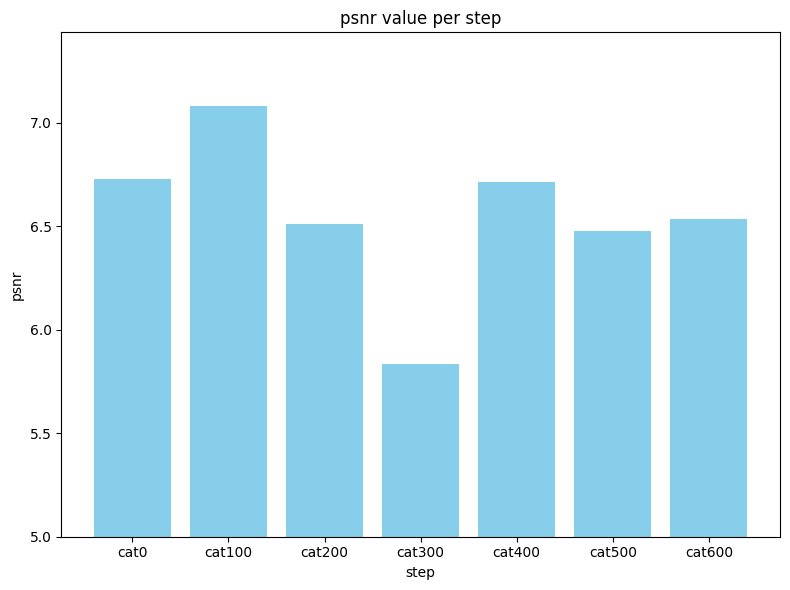
\includegraphics[width=\linewidth]{images/pixel-psnr.png}
    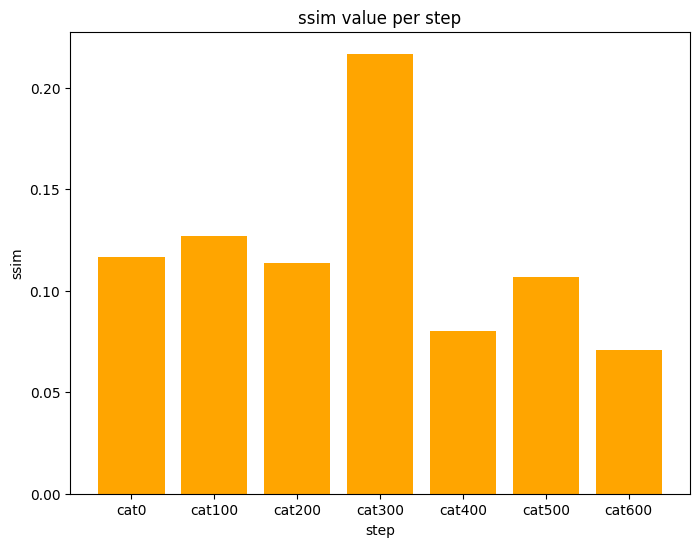
\includegraphics[width=\linewidth]{images/pixel-ssim.png}
	\caption{
		PSNR and SSIM result of pixel illustration LoRA by step size.}
	\vspace{-2mm}
        \label{fig:pixelchart}
\end{figure}

\begin{figure}[t]
\centering
	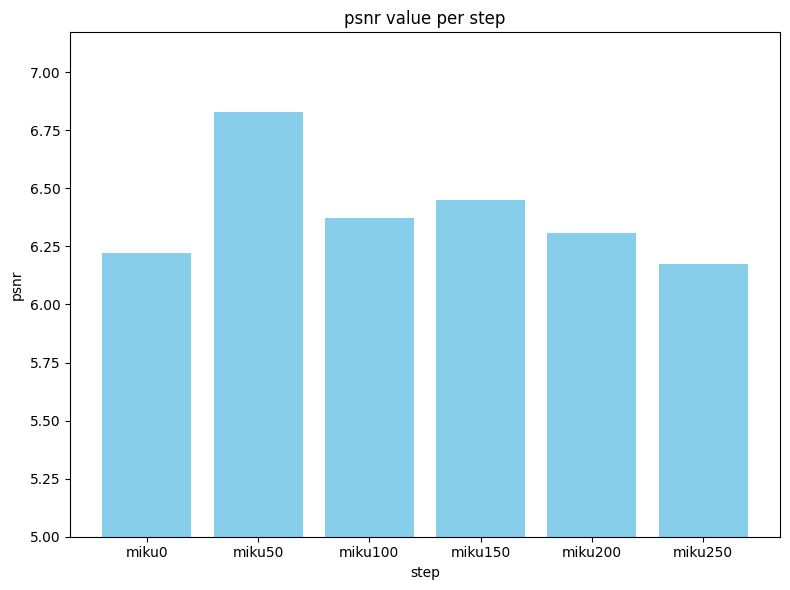
\includegraphics[width=\linewidth]{images/miku-psnr.png}
    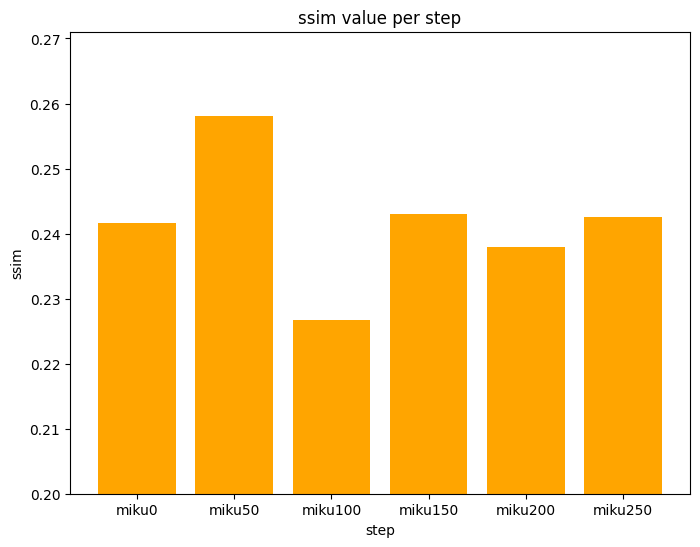
\includegraphics[width=\linewidth]{images/miku-ssim.png}
	\caption{
		PSNR and SSIM result of Hatsune Miku LoRA by step size.}
	\vspace{-2mm}
        \label{fig:mikuchart}
\end{figure}

\begin{figure}[t]
\centering
	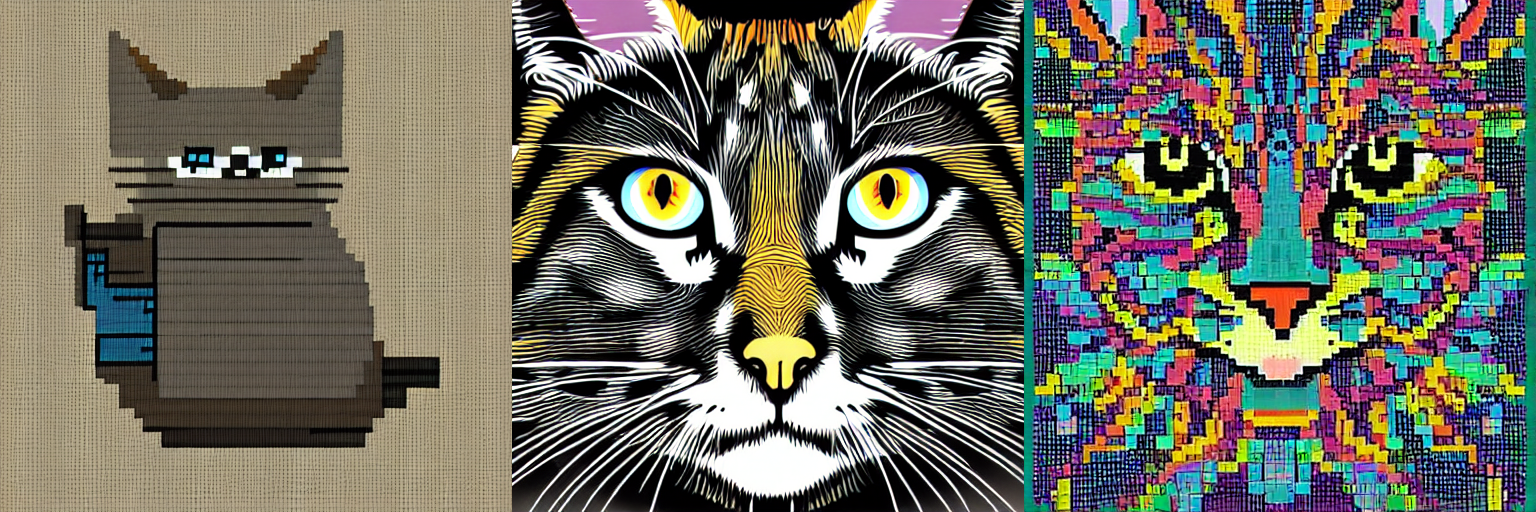
\includegraphics[width=\linewidth]{images/cat0.png}
    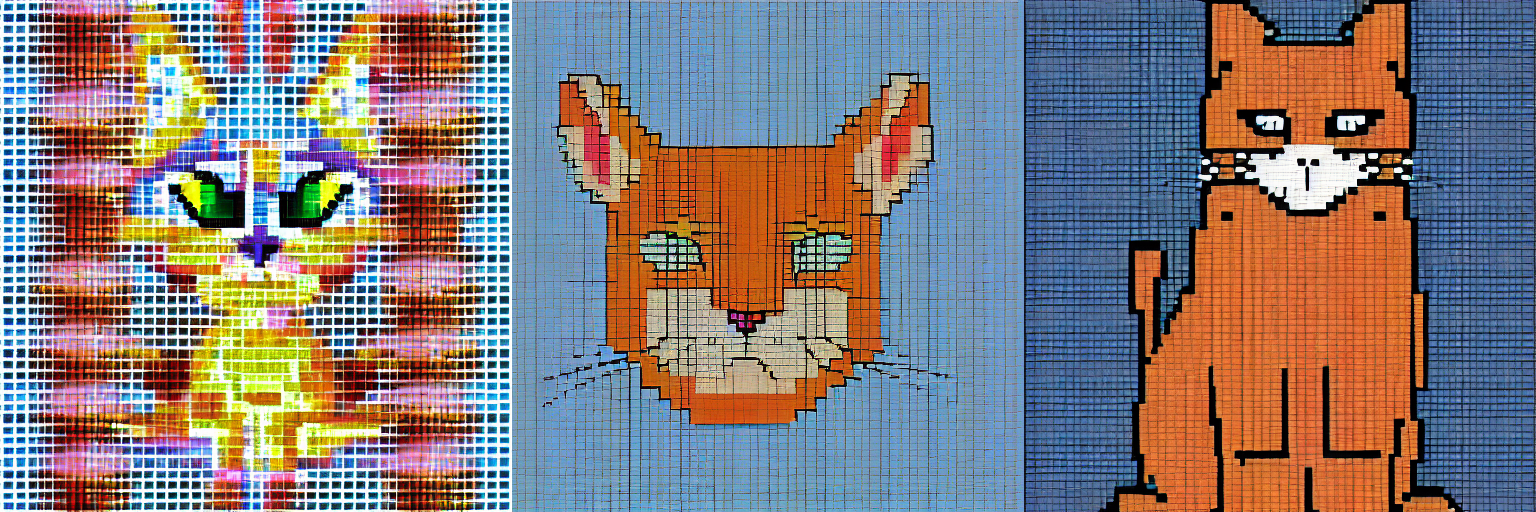
\includegraphics[width=\linewidth]{images/cat100.png}
    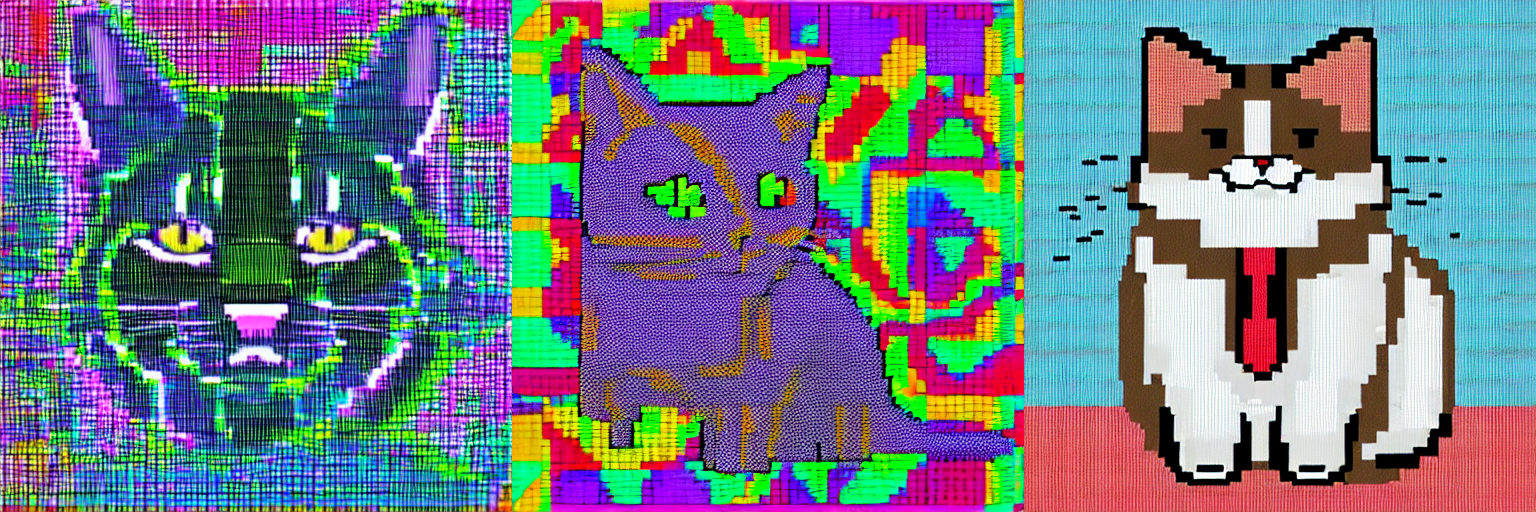
\includegraphics[width=\linewidth]{images/cat200.png}
    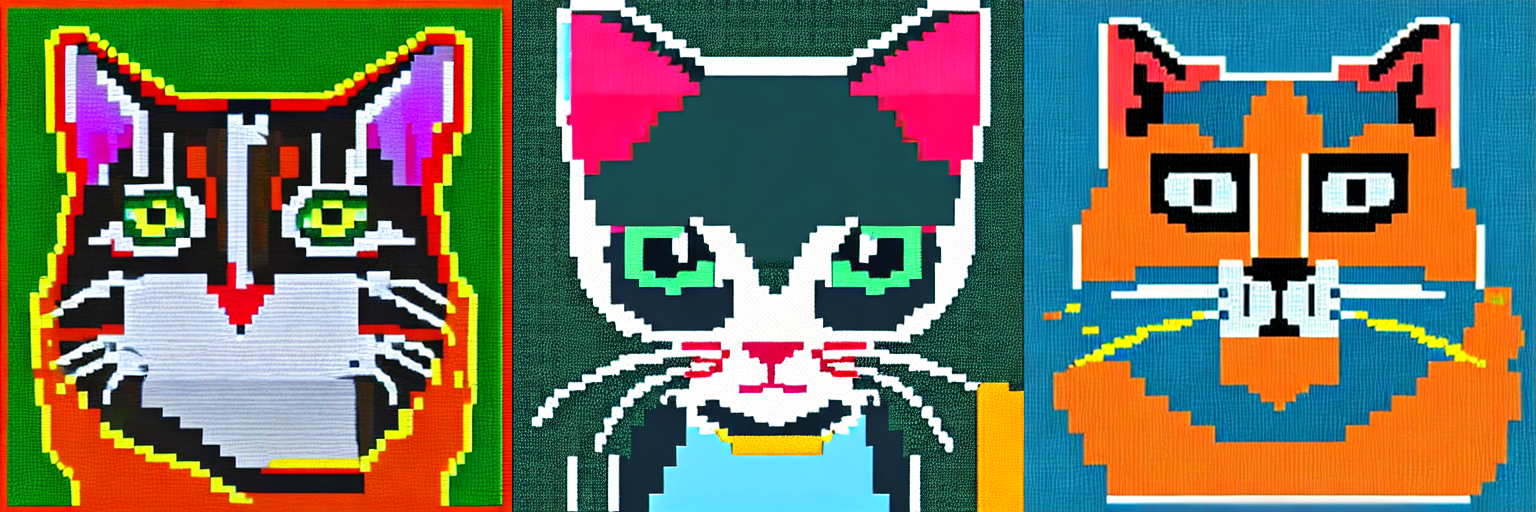
\includegraphics[width=\linewidth]{images/cat300.png}
    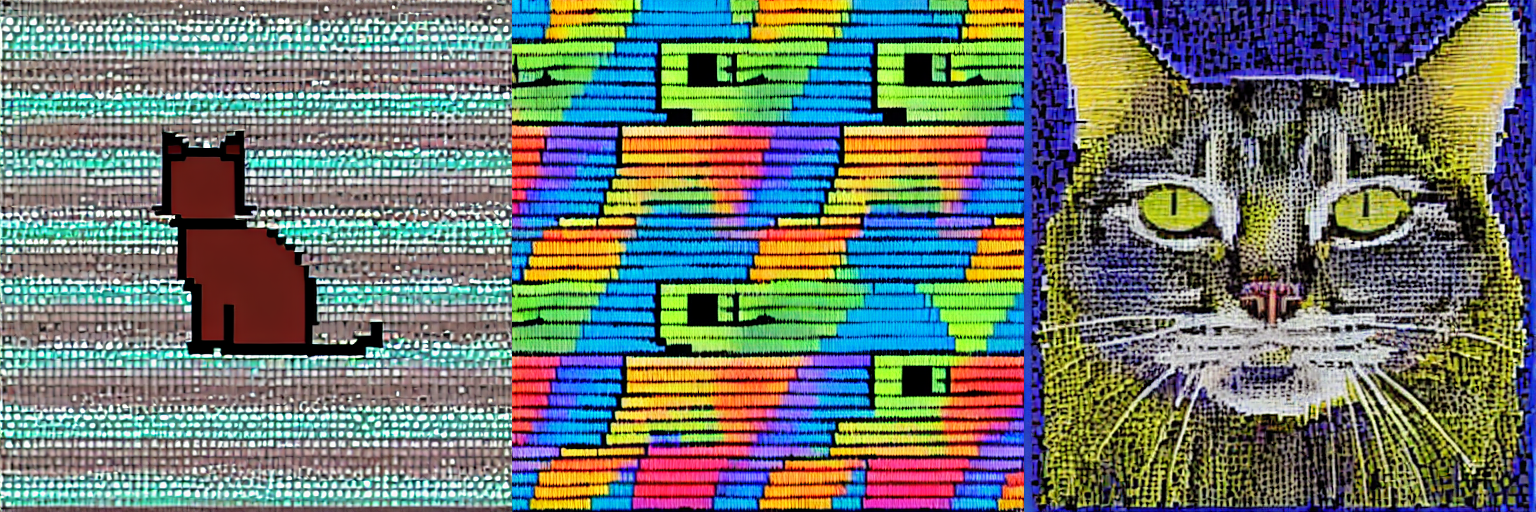
\includegraphics[width=\linewidth]{images/cat400.png}
    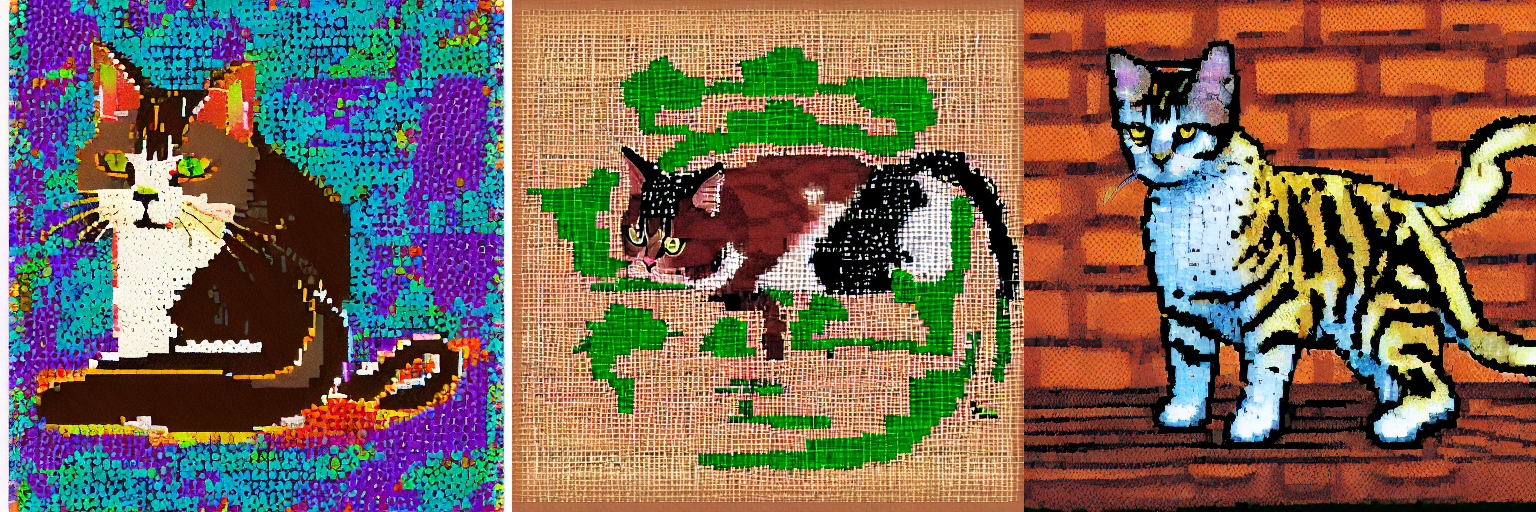
\includegraphics[width=\linewidth]{images/cat500.png}
    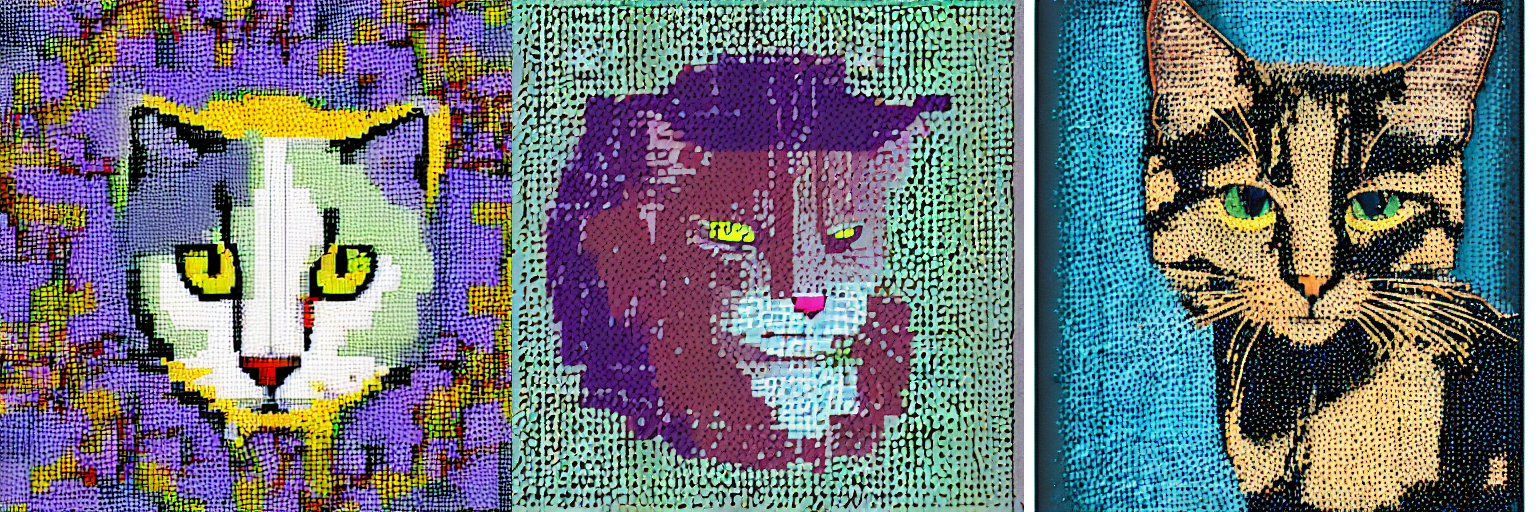
\includegraphics[width=\linewidth]{images/cat600.png}
	\caption{
		Inference of the Pixel Illustration LoRA model integrated with Stable Diffusion by varying the number of training steps. The training parameters were consistently maintained across experiments. the text prompt is 'pixel illustration of cat'. The figure shows a inference result from top to bottom, starting without applying LoRA and subsequently showing results at 100, 200, 300, 400, 500, and 600 steps.}
	\vspace{-2mm}
        \label{fig:pixelresult1}
\end{figure}

\begin{figure}[t]
\centering
	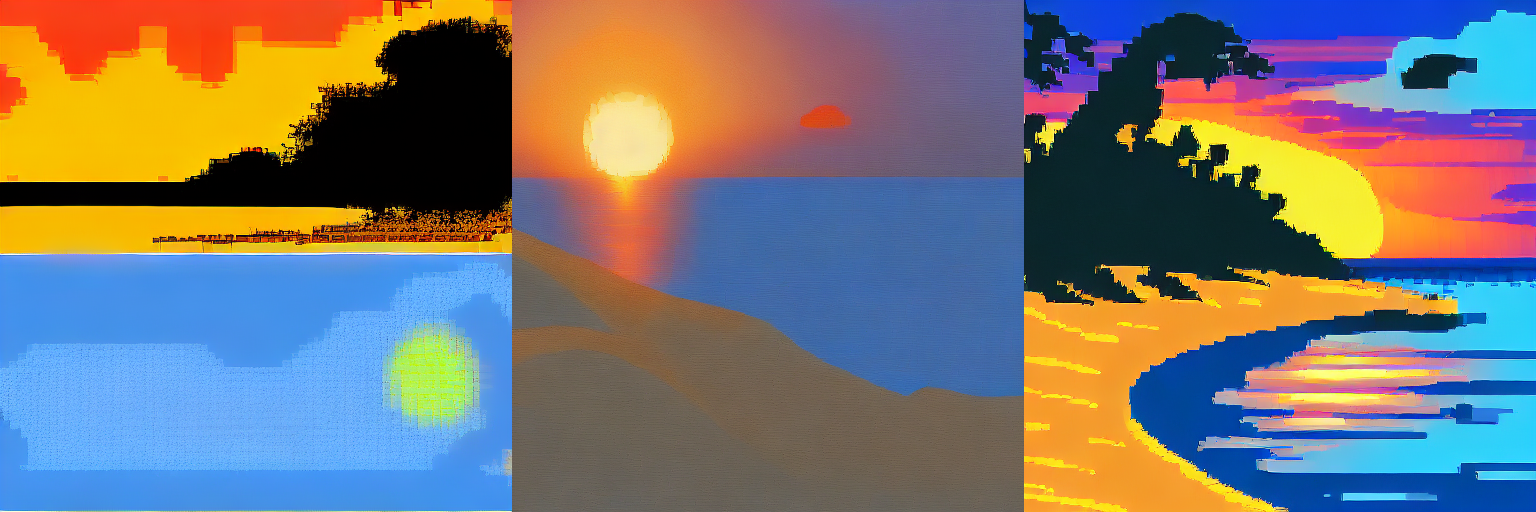
\includegraphics[width=\linewidth]{images/beach sunset500.png}
    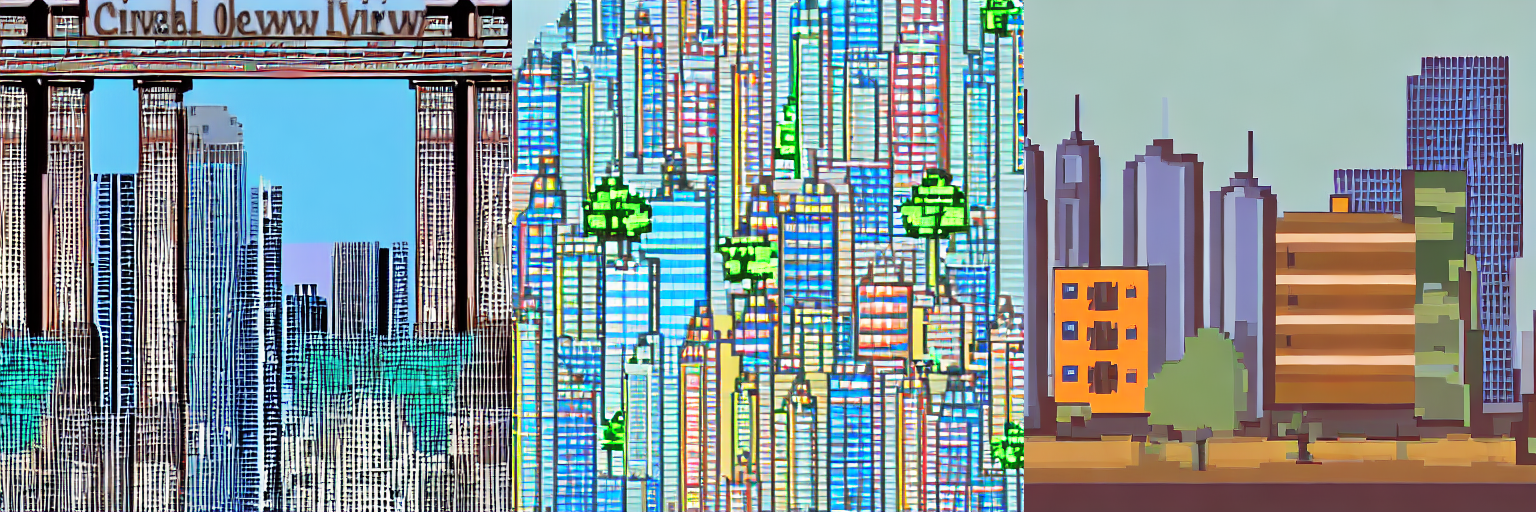
\includegraphics[width=\linewidth]{images/city500.png}
    
	\caption{
		Inference of the Pixel Illustration LoRA model integrated with Stable Diffusion with 500 training steps. The training parameters were consistently maintained across experiments. The text prompt of the first image is 'illustration of beach and sunset', and second image is 'illustration of cityview'}
	\vspace{-2mm}
        \label{fig:pixelresult2}
\end{figure}

\begin{figure}[t]
\centering
	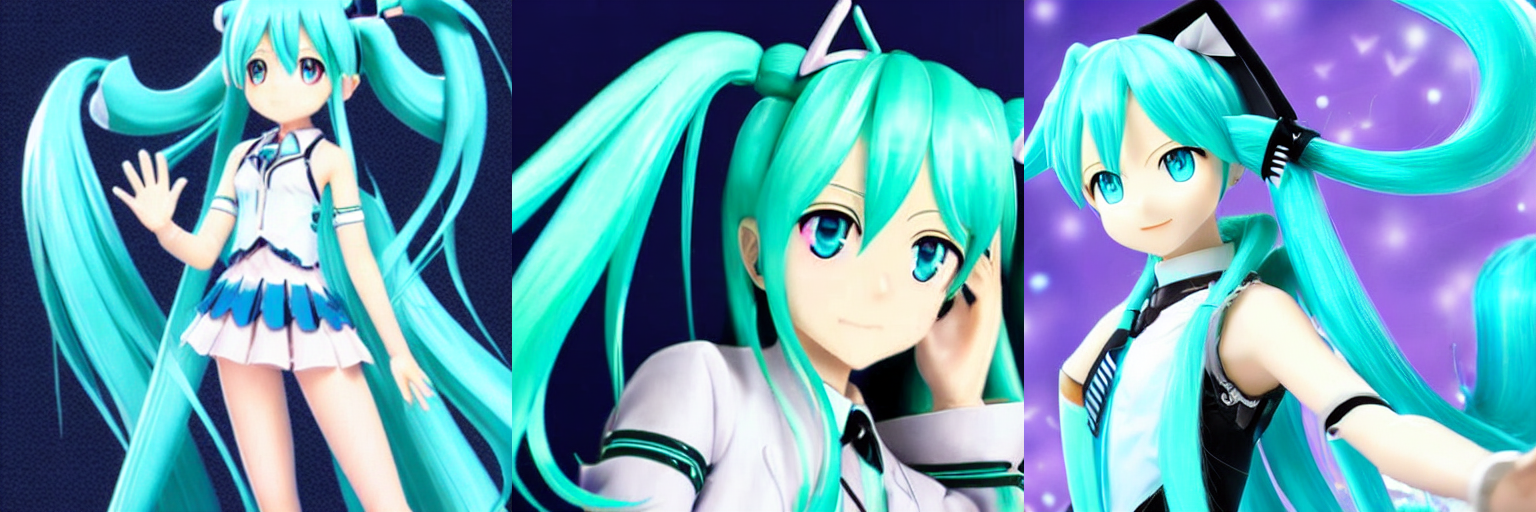
\includegraphics[width=\linewidth]{images/miku0.png}
    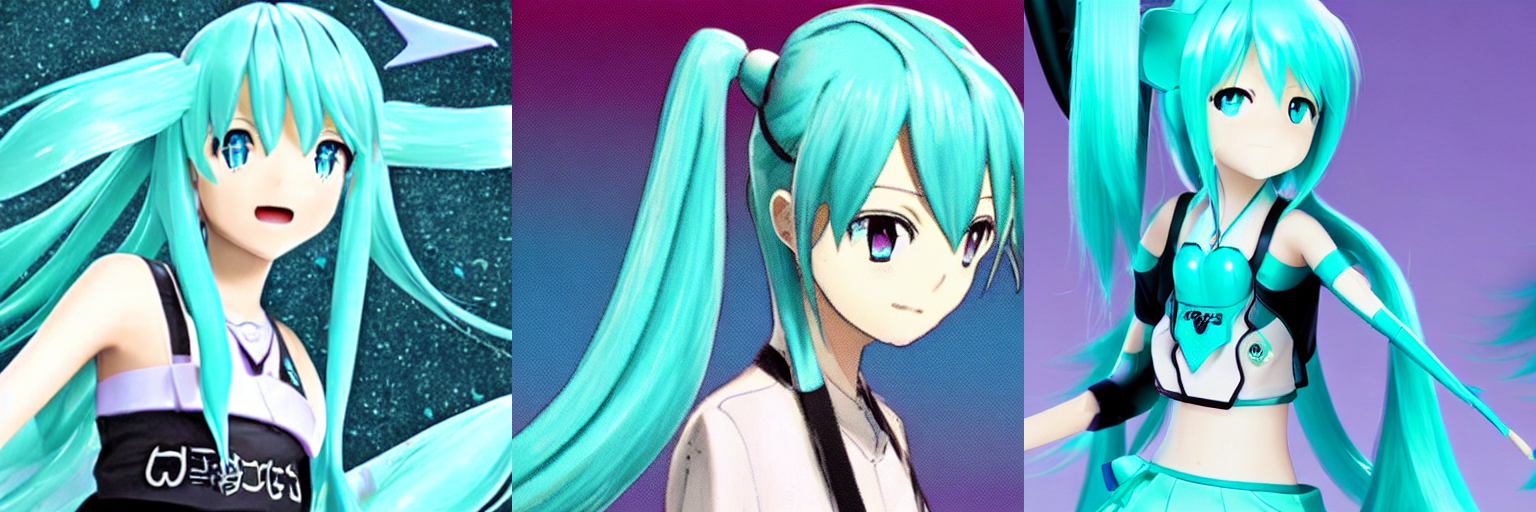
\includegraphics[width=\linewidth]{images/miku50.png}
    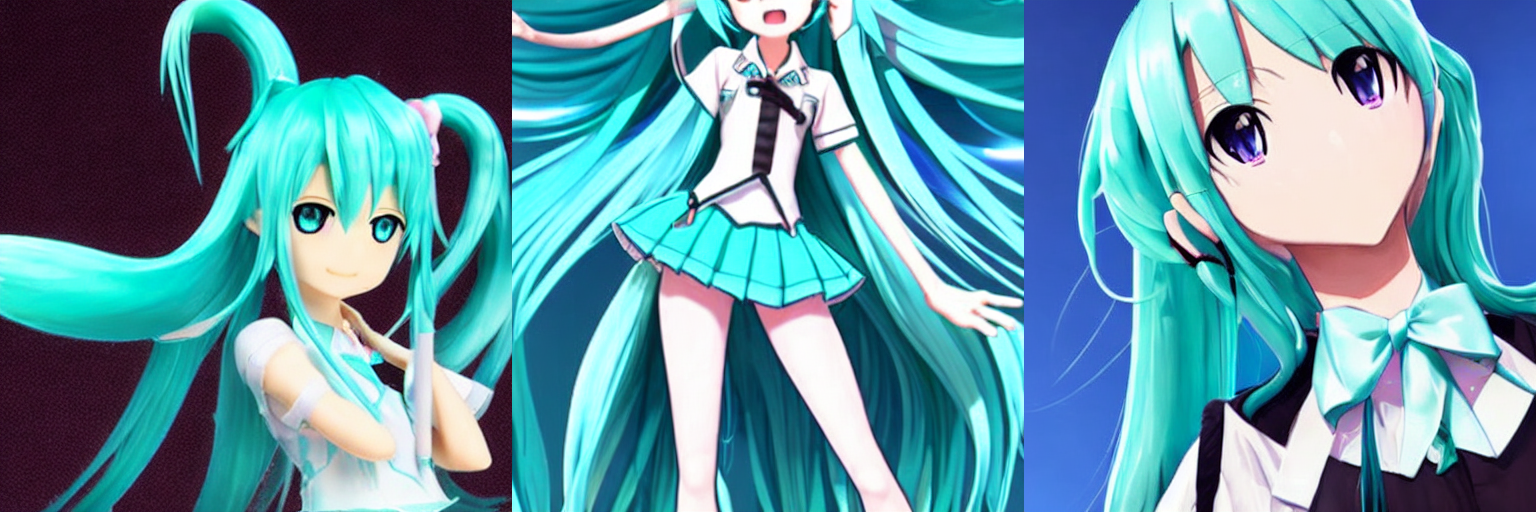
\includegraphics[width=\linewidth]{images/miku100.png}
    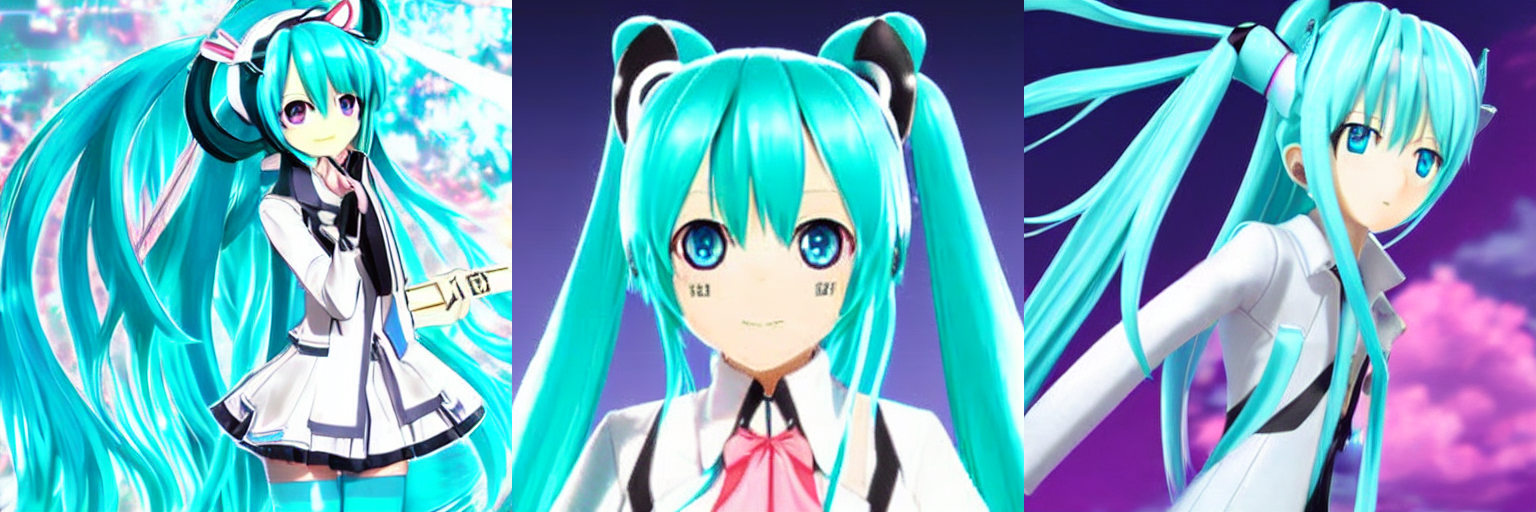
\includegraphics[width=\linewidth]{images/miku150.png}
    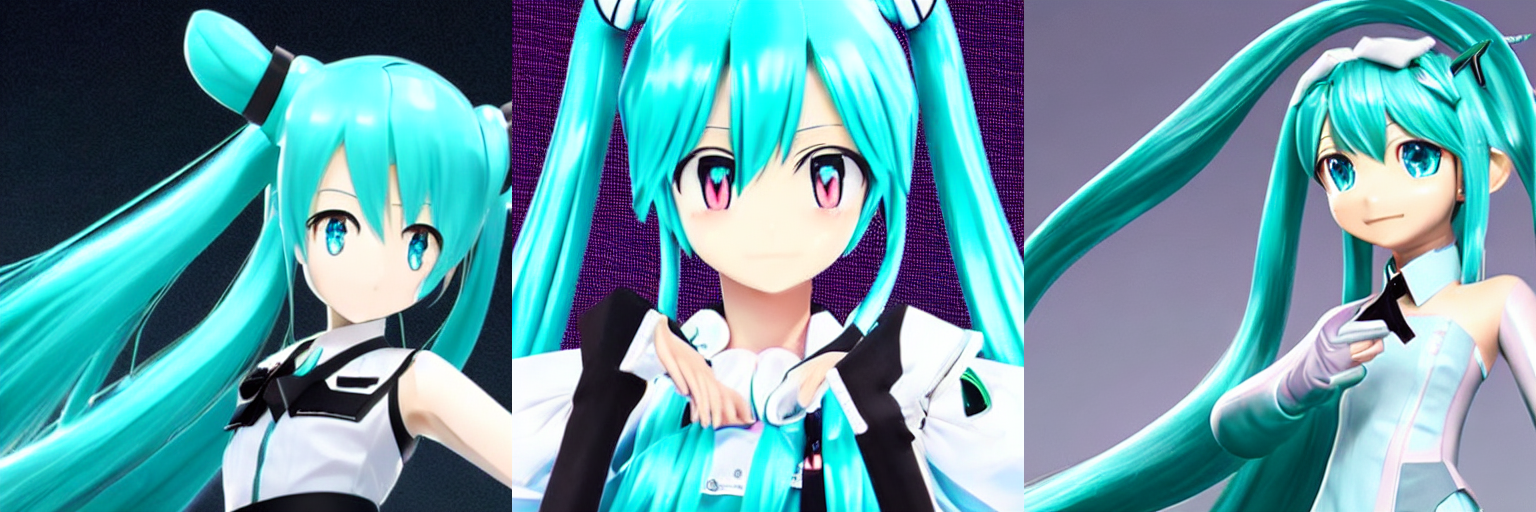
\includegraphics[width=\linewidth]{images/miku200.png}
    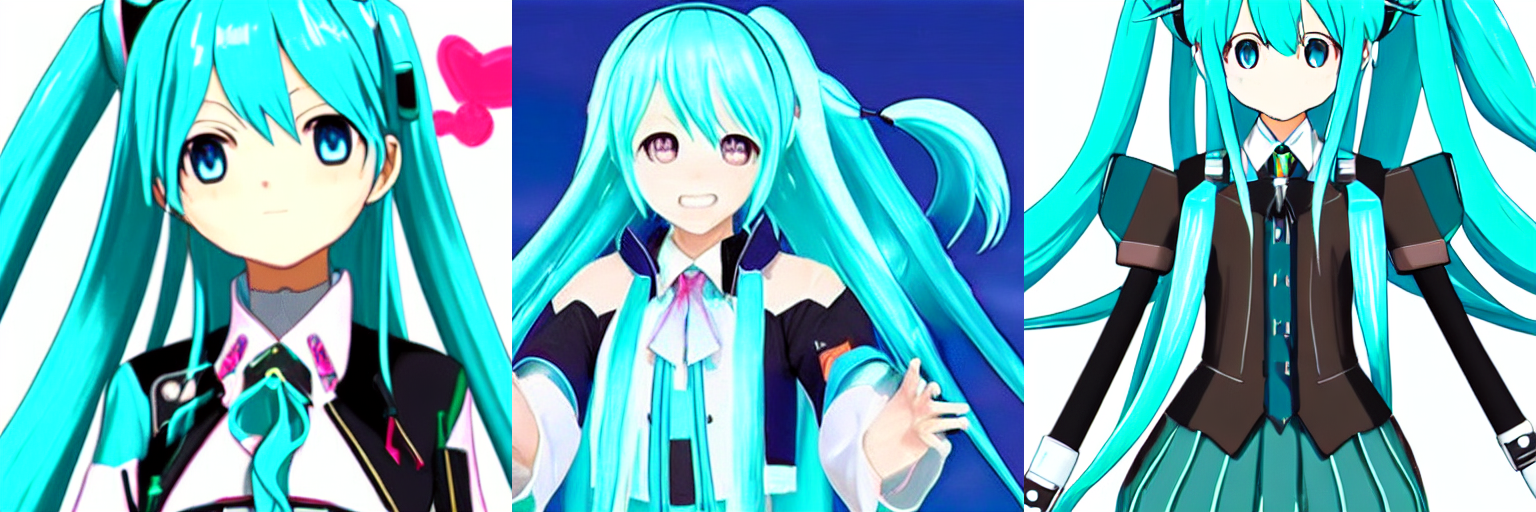
\includegraphics[width=\linewidth]{images/miku250.png}
    
	\caption{
		Inference of the Hatsune Miku LoRA model integrated with Stable Diffusion by varying the number of training steps. The training parameters were consistently maintained across experiments. the text prompt is 'hatsune miku'. The figure shows a inference result from top to bottom, starting without applying LoRA and subsequently showing results at 50, 100, 150, 200, and 250}
	\vspace{-2mm}
        \label{fig:mikuresult}
\end{figure}

\newpage
\bibliography{egbib}
\appendix
\section{Applying various LoRA weights available on Hugging Face Hub.}

On the Hugging Face Hub, many people have uploaded LoRA weights trained on a variety of datasets. In this section, We will explain how to apply LoRA weights on Stable Diffusion XL. 
You can search for various LoRA weights on \href{https://huggingface.co/models?other=base_model:stabilityai/stable-diffusion-xl-base-1.0}{Hugging Face Hub}. Before running the code below, PyTorch and Diffusers must be installed. this code creates stable diffusion XL pipeline, initializes weights with pretrained model, reduces memory usage by applying FP16 precision.

\begin{verbatim}
import torch
from diffusers import StableDiffusionXLPipeline
    as pline
from diffusers.utils import
    make_image_grid

pid = "stabilityai/stable-diffusion-xl-base-1.0"
device = torch.device("cuda") // for nvidia gpu
//device=torch.device("cpu") // for cpu
pipeline = pline.from_pretrained(
    pretrained_model_name_or_path = pid,
    torch_dtype = torch.float16,
    variant = "fp16",
    use_safetensors = True,
    ).to(device)

\end{verbatim}
After creating pipeline, you can load the LoRA weights using the name of the LoRA weights.
\begin{verbatim}
pipeline.load_lora_weights("user/lora-weight-name")
\end{verbatim}

Additionally, you can unload the current weights and load different LoRA weights.

\begin{verbatim}
pipeline.unload_lora_weights()
pipeline.load_lora_weights("user/other-lora-weights")
\end{verbatim}

You can also load multiple LoRA models simultaneously. Each LoRA weight can be loaded by specifying an adapter name when loading them.

\begin{verbatim}
pipeline.unload_lora_weights()
pipeline.load_lora_weights("TheLastBen/Papercut_SDXL", 
    adapter_name="paper_cut")
pipeline.load_lora_weights("nerijs/pixel-art-xl", 
    adapter_name="pixel_art")
pipeline.set_adapters(["paper_cut", "pixel_art"], 
    adapter_weights=[0.5, 1.0])
\end{verbatim}

After the LoRA weights are loaded, you can generate images similar to the images, styles, or characters the LoRA was trained on. The code below generates 3 images of "lego minifig of a kpop idol" with the LoRA weights.

\begin{verbatim}
prompt = "lego minifig of a kpop idol"
images= pipeline(prompt,num_images_per_prompt=3).images
make_image_grid(images, rows=1, cols=3)
\end{verbatim}
An example of images generated by applying LoRA weights to Stable Diffusion XL is shown in Figure \ref{fig:loraxlresult1}, \ref{fig:loraxlresult2} and \ref{fig:loraxlresult3}.

\begin{figure}[t]
\centering
	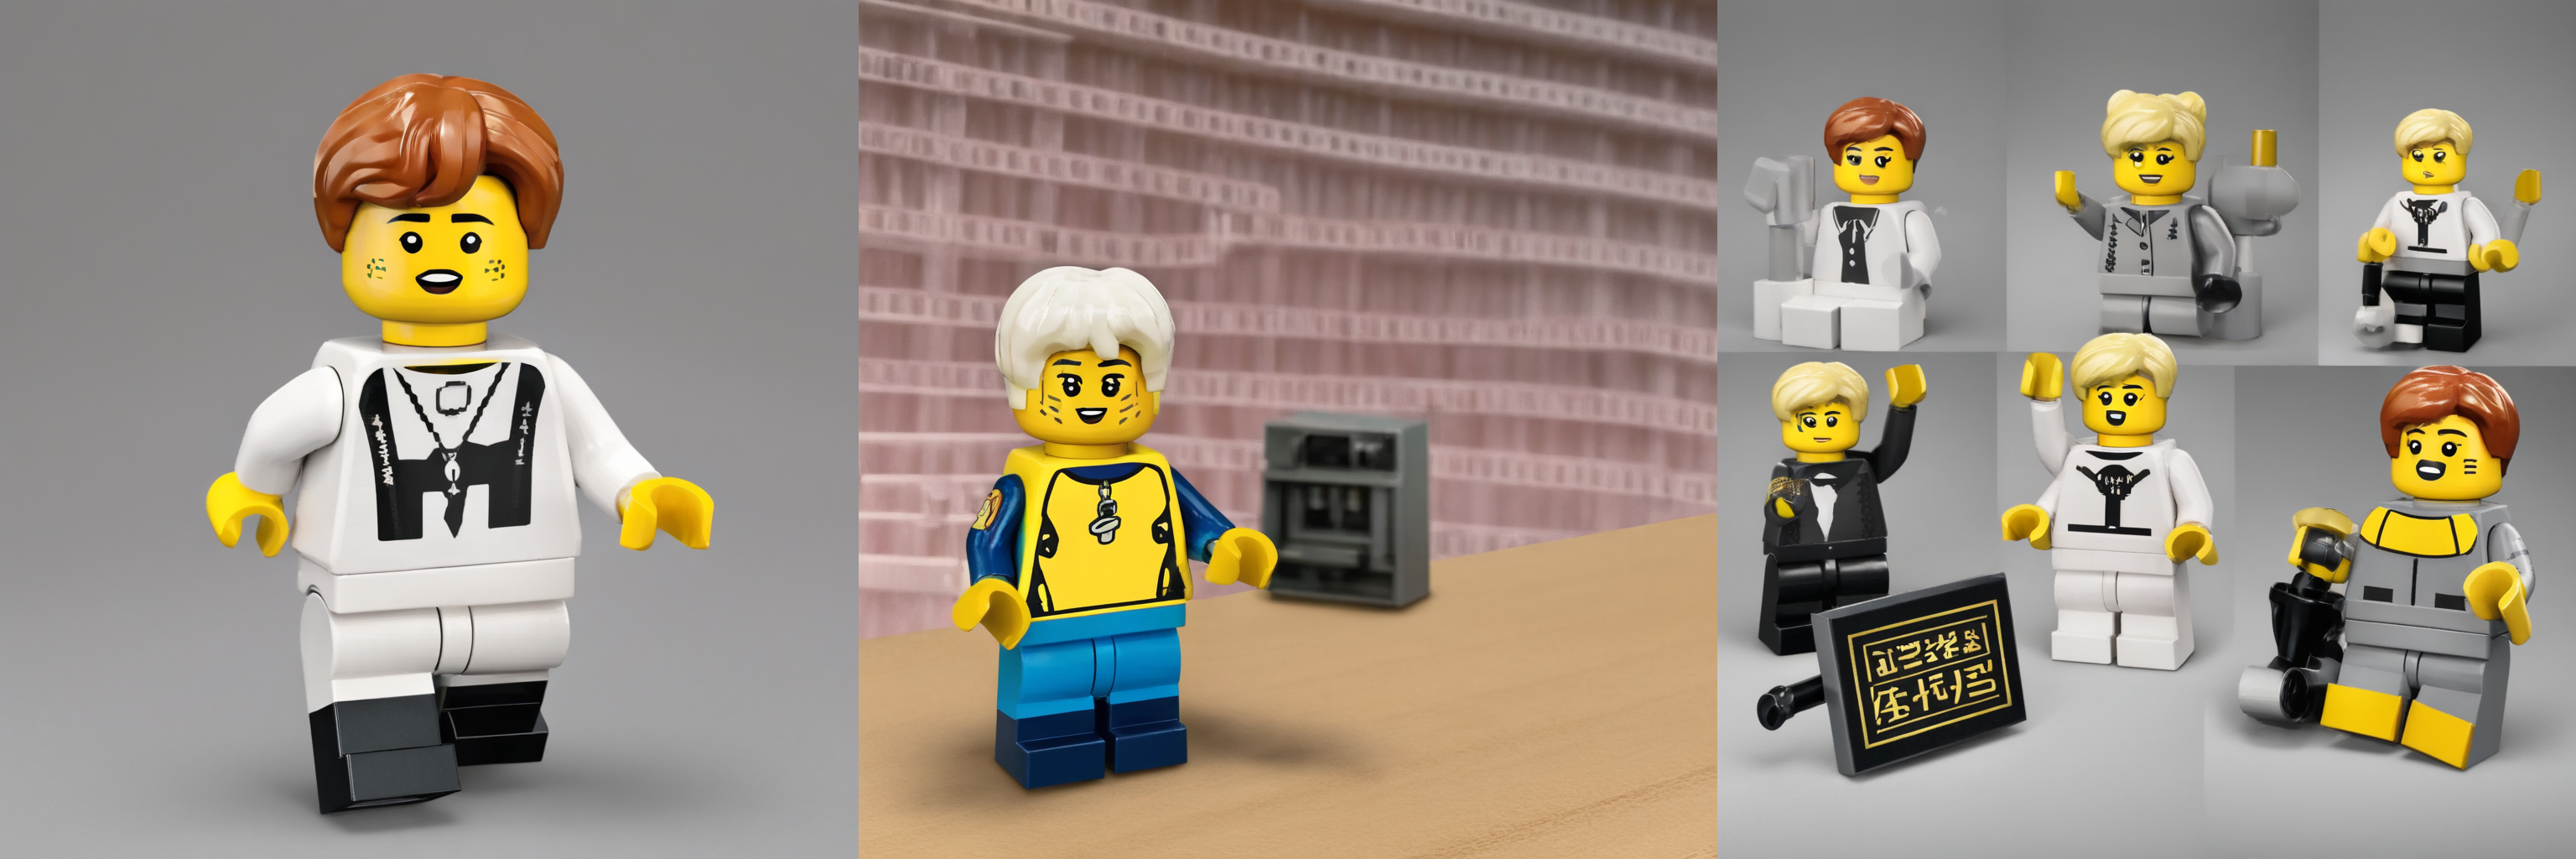
\includegraphics[width=\linewidth]{images/xlkpopidol.png}
    
    
	\caption{
		Inference of the nerijs/lego-minifig-xl LoRA integrated with Stable Diffusion XL. the prompt is 'lego minifig of a kpop idol'}
	\vspace{-2mm}
        \label{fig:loraxlresult1}
\end{figure}

\begin{figure}[t]
\centering
	
\includegraphics[width=\linewidth]{images/xl3d.png}
    
    
	\caption{
		Inference of the goofyai/3d\_render\_style\_xl LoRA integrated with Stable Diffusion XL. the prompt is '3d style of a man with a hat'}
	\vspace{-2mm}
        \label{fig:loraxlresult2}
\end{figure}

\begin{figure}[t]
\centering
	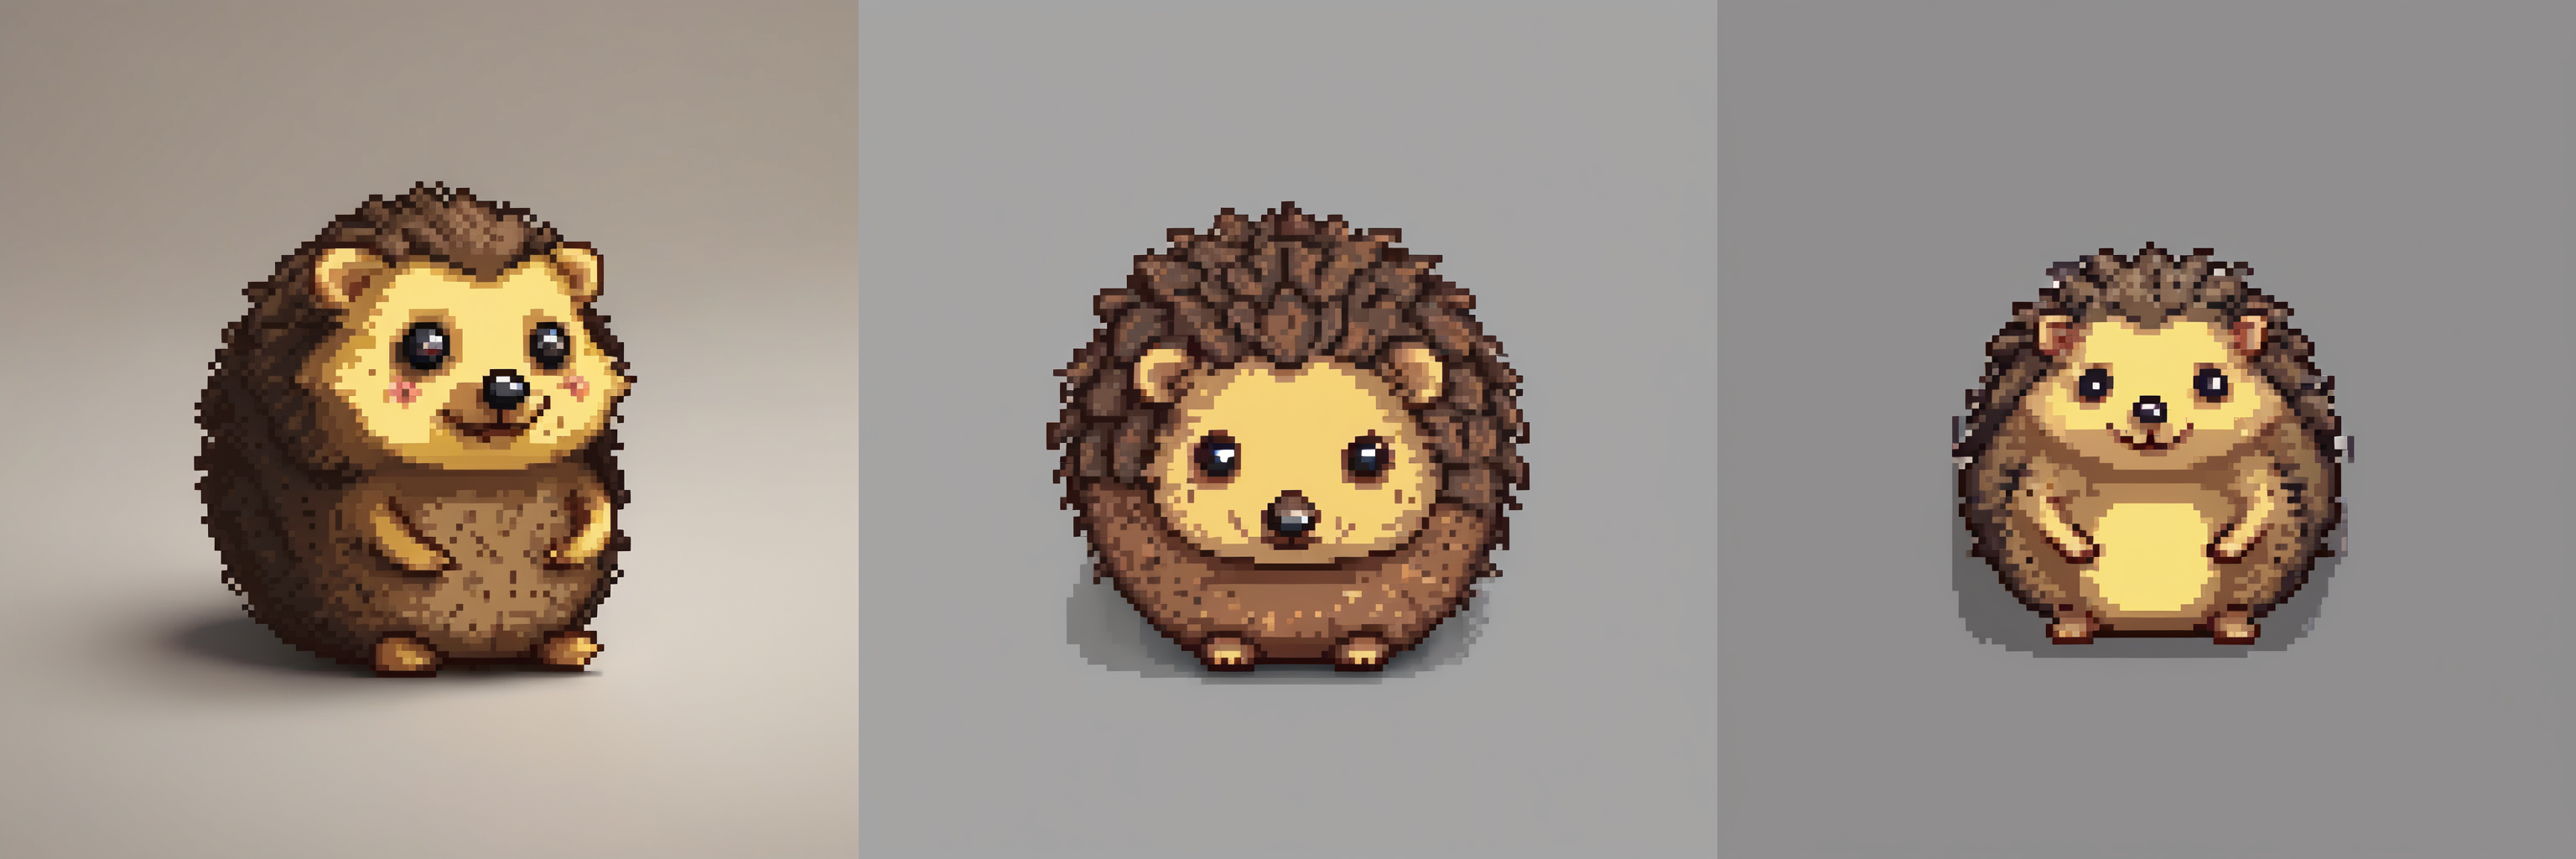
\includegraphics[width=\linewidth]{images/xlpixel.png}
    
    
	\caption{
		Inference of the TheLastBen/Papercut\_SDXL and nerijs/pixel-art-xl LoRA integrated with Stable Diffusion XL. the prompt is 'A cute hedgehog plushie with a brown back and yellow face with black eyes, pixel art, paper cut'. Each LoRA adapter weights are 0.5 and 1.0, respectively.}
	\vspace{-2mm}
        \label{fig:loraxlresult3}
\end{figure}
\section{Good prompt}
A prompt is a key sentence that guides an AI model to generate the desired image. An effective prompt helps the model clearly and precisely understand the image you want. Good prompt should contains subject, character, action, location and emotion. 

Additionally, color, texture, proportions, perspective, reflection and shadows add specific details that enhance the depth and richness of the image. For example, 'A man with a hat sitting on a bench in a bustling city park, looking contemplative, pastel tone color, rough texture, close up, low angle, low contrast' is a detailed prompt.

Artistic style is also add an information of desired images. For example, Comic Book, Watercolor, Oil Painting and Pencil Sketch is good artistic style prompt.

A negative prompt specifies that certain elements should be excluded from the generated image. For example, worst quality, low quality, jpeg artifacts and blurry is good negative prompts.

you can specify the negative prompt using the code below: 
\begin{verbatim}
advanced_image_4 = pipeline(
    prompt=advanced_prompt_2,
    prompt_2=advanced_prompt_3,
    negative_prompt=negative_prompt_1,
    negative_prompt_2=negative_prompt_2,
    num_images_per_prompt=1,
).images[0]

\end{verbatim}

Guidance scale and step are parameters that influence image generation. The default value of the Guidance Scale is 5. The higher the value, the stronger the influence of the prompt; the lower the value, the weaker the influence of the prompt. The step refers to the number of steps required to generate an image. The default value is 50. Increasing the step value will produce higher-quality images, but it will take more time.

\begin{verbatim}
    advanced_image_8 = pipeline(
    prompt=advanced_prompt_2,
    prompt_2=advanced_prompt_3,
    negative_prompt=negative_prompt_1,
    negative_prompt_2=negative_prompt_2,
    guidance_scale=5,
    num_inference_steps=100,
    num_images_per_prompt=1,
).images[0]
\end{verbatim}

\section{Stable Video Diffusion}
Stable Video Diffusion\cite{videodiffusion} takes a single image as input and generates intermediate frames to create a short video.
you can generate the video using the code below:
\begin{verbatim}
from diffusers import 
    StableVideoDiffusionPipeline
from diffusers.utils import 
    export_to_gif

pipe = StableVideoDiffusionPipeline.from_pretrained(
    "stabilityai/stable-video-diffusion-img2vid-xt",
    torch_dtype=torch.float16,
    variant="fp16",
)
pipe.enable_model_cpu_offload()
frames = pipe(image, 
    decode_chunk_size=15).frames[0]
export_to_gif(frames, "test.gif")

\end{verbatim}

\section{other ways to training LoRA}
Using the Diffusers and Accelerate library, you can train LoRA in a CLI environment. The document is \href{https://huggingface.co/docs/diffusers/en/training/lora}{here}

Additionally, Thanks to kohya\_ss library made by bmaltais, you can train LoRA in a GUI environment. The code and documents are \href{https://github.com/bmaltais/kohya_ss}{here}

There are also various AI art-related communities where you can receive support, share your creations, and connect with other enthusiasts. Here are some notable ones:
\begin{itemize}
    \item \href{https://www.reddit.com/r/StableDiffusion/}{r/StableDiffusion}
    \item \href{https://www.reddit.com/r/aiArt/}{r/aiArt}
    \item \href{https://arca.live/b/hypernetworks}{AI Picture Training Channel (arca.live)}
\end{itemize}

\end{document}


